%5 提案手法
\section{提案手法}
本研究の目的は移動を伴う環境において,テレイグジスタンスにより遠くにいる友人と,あたかも遠隔地で行動しているかのような体験を可能とする手法を提案し,提案手法を基に移動しながら遠くにいる友人と遠隔旅行をするシステムを開発することである.目的実現のために他ユーザの表示と遠隔地の風景表示を行う.
しかし移動しながらシステムを使用する場合に達成すべき課題が2つある.
1つはシステムを使用する際に周囲の環境を認識できることである.
本手法では遠隔地の風景を表示する際に道路部分は現実の風景を表示し,道路以外の部分のみ遠隔地の風景を表示することでユーザが周囲の状況を把握しながら遠隔存在することを可能にする.
2つ目はユーザがどれだけ移動しても遠隔地でユーザの存在が投影され続けることである.そのため本手法では自身の存在を遠隔地に投影させるために自分の3Dモデルではなくアバターを遠隔地に投影することでカメラの撮影範囲などの移動制限を無くし現実環境を際限なく移動可能にする.
これらの手法を実装したシステムによって遠くにいるユーザと遠隔旅行をする際,実際に移動しながらの体験が可能となる.

%我々はこれらの手法の有効性を評価するため,遠隔地の風景での行動を遠くにいる友人と共に体験することを可能にするシステムを開発した.
%開発したシステムはMRを用いて他ユーザをアバターとして表示し,遠隔地風景のパノラマ画像を表示する.
%これにより遠隔地の風景を見ながら表示された他ユーザのアバターと共に行動ができる.
\clearpage

\subsection{他ユーザの表示}
遠くにいる他ユーザを表示することで,1人で行動する際にあたかも複数人で一緒に行動しているかのような体験を可能にする.

%遠くにいる友人と行動しているかのような体験をするために,離れた場所にいる他ユーザのアバターを表示する.
\subsubsection{アバターの表示}
遠くにいる他ユーザを表示する際自身の3Dモデルなどではなくバーチャルヒューマンをユーザのアバターとして表示することで,自分自身の3Dモデル生成するためにカメラやKinect\cite{kinect}に写る必要がなくなる.その結果制限無く自由に移動することが可能となる.%本手法で扱うアバターはバーチャルヒューマンと呼ばれその存在が人の認知に対し影響を与えることがわかっている\cite{virtualhuman}.

\subsubsection{表示する他ユーザの選択}
表示する他ユーザは自分と同じ場所を遠隔地として指定したかによって選択する.
図\ref{figure:avatershare}は2人のユーザが同じ場所を遠隔地として指定した時の例である.
名古屋にいるユーザ1が遠隔地として指定したローマのコロッセオを,ロサンゼルスにいるユーザ2も同様に遠隔地として指定しているため,ユーザ1の視点には遠くにいるユーザ2のアバターが見える.逆も同様である.これにより他ユーザと一緒に行動することが可能となる.
%ユーザ同士のマッチングをユーザが指定した遠隔地の座標を比較し,距離が近いユーザがいた場合に行う.そしてマッチングされたユーザのアバターを表示する.
この時のユーザ同士を引き合わせる処理はオンラインゲームでRoomと呼ばれるサーバにユーザを接続し同期処理を行うPhoton Unity Cloud を利用した\cite{photon}.
これによりユーザはあたかも複数人でいるかのように感じることが可能となる.

\begin{figure}[htbp]
\begin{center}
\includegraphics[width=11cm]{img/02_proposedmethod/shareava.eps} 
\end{center}
\caption{他ユーザのアバター表示}
\label{figure:avatershare}
\end{figure} 

\clearpage

\subsubsection{アバターの動き}
アバターとユーザの位置と向きを同期することで,ユーザが移動した際にアバターも同様に移動する.ユーザとアバターの同期はヘッドマウントディスプレイの自己位置推定機能を用いて取得した端末の座標と方向を用いて行う.
この時アバターの方向は水平方向の変化のみ同期する.これによりユーザが上を見上げた時アバターが倒れることを防ぐ.

\clearpage





%\begin{figure*}[t]
%\begin{center}
%\includegraphics[width=17cm]{img/useimage.eps} 
%\end{center}
%\caption{風景重畳:(a)遠隔地の設定画面.(b)システムを使用イメージ.(c)出力イメージ}
%\label{figure:useimage}
%\end{figure*} 

\subsection{風景重畳}
%またユーザが風景を見る時は実際に歩くため,身体的動作の不一致によるVR酔いを抑制できる.
遠隔地で行動しているかのような体験をするために遠隔地の風景を360度パノラマ画像として取得し道路部分を切り抜き現実の風景に重畳表示する.これによりユーザの周囲の風景の道路以外の部分を変化させる.図\ref{figure:changescenery}に本手法を用いて豊田市の風景に対し,ローマのコロッセオの風景を重畳した例を示す.現実地風景(豊田市)は道路以外の部分が切り抜かれ,遠隔地風景(ローマのコロッセオ)は道路部分が切り取られている.切り取りを行なった2つの風景を重畳することで道路部分は現実地風景(豊田市),道路以外の部分は遠隔地風景(ローマのコロッセオ)が表示される.

\begin{figure}[htbp]
\begin{center}
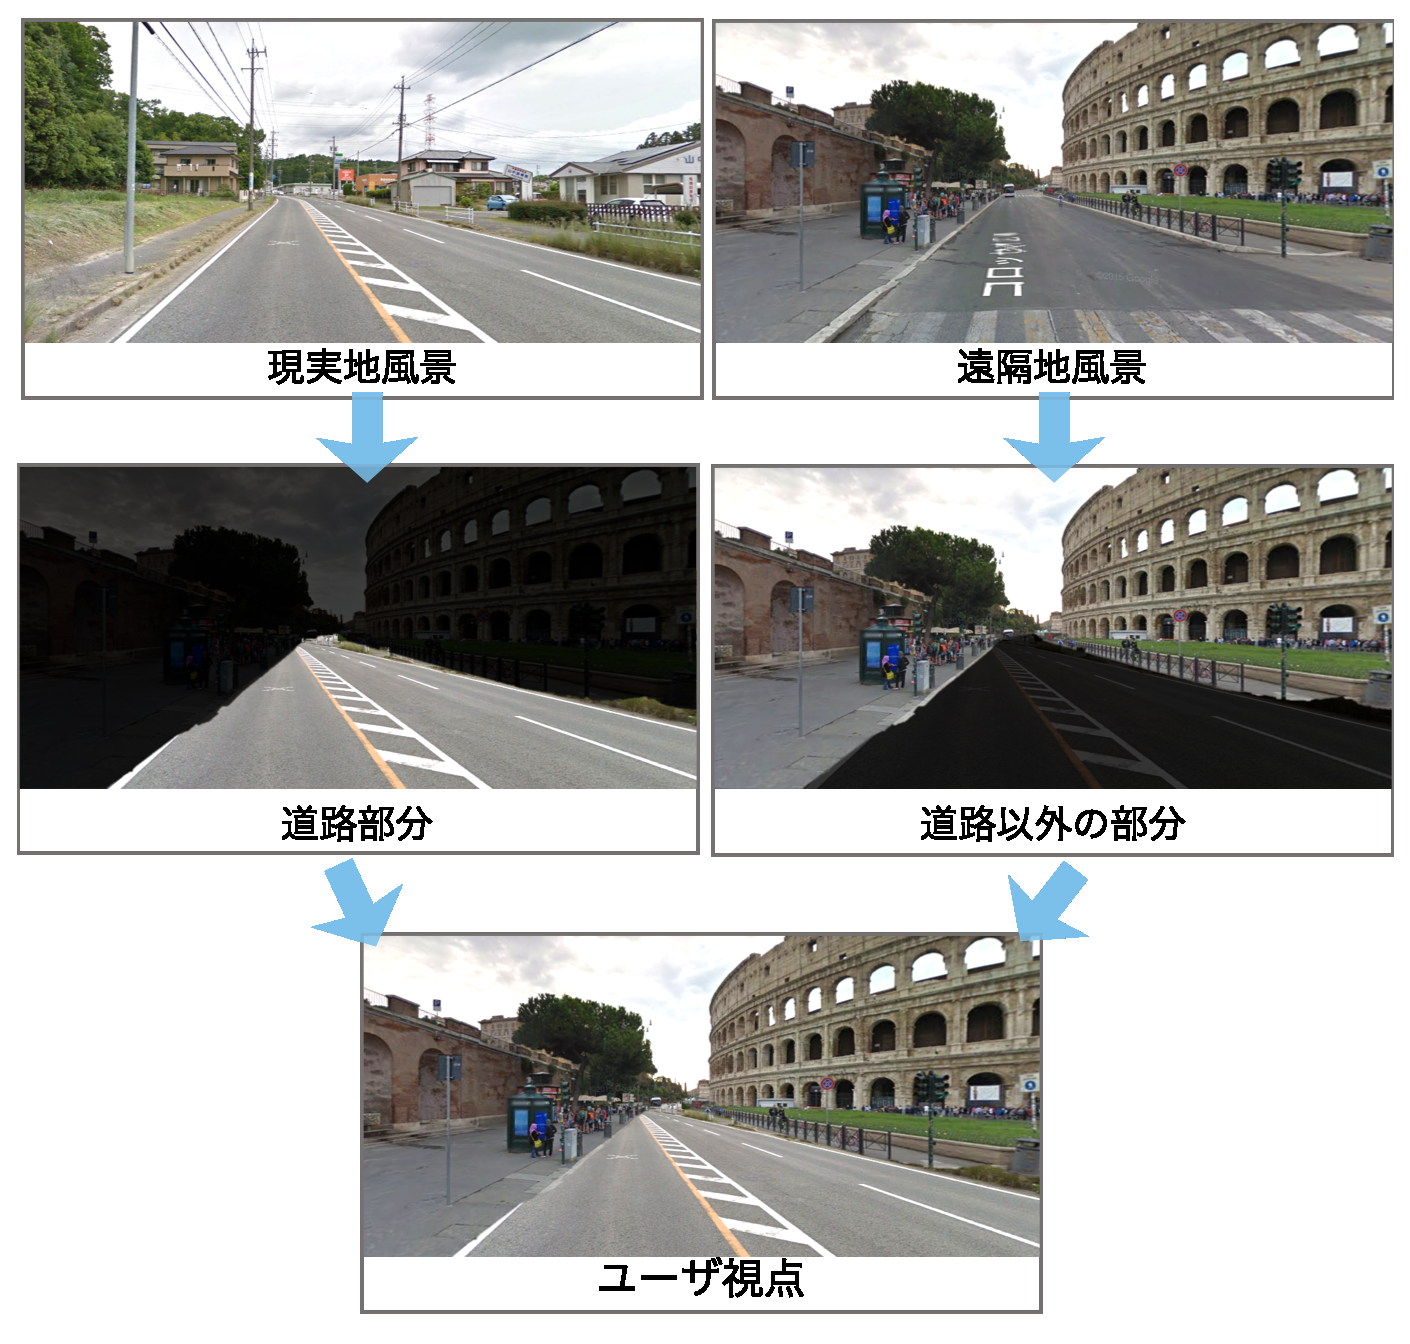
\includegraphics[width=11cm]{img/02_proposedmethod/changescenery.eps} 
\end{center}
\caption{風景変化}
\label{figure:changescenery}
\end{figure} 

\clearpage


\subsubsection{風景表示}
遠隔地の360度パノラマ画像を用いてユーザ周囲の風景を変化させる.パノラマ画像は GoogleStreetView\cite{gsv} を複数の視線の向きで取得した画像を結合することで取得する.
取得したパノラマ画像を球体型のオブジェクトの表面にテクスチャとして貼り付け,球体オブジェクトの内側に視点を置く事で周囲の風景を変化させる.ローマのコロッセオのパノラマ画像を生成し,球体オブジェクトに貼り付け内側から見た様子を図\ref{figure:sphere}に示す.

\begin{figure}[htbp]
\begin{center}
\includegraphics[width=16cm]{img/02_proposedmethod/scenery_change.eps} 
\end{center}
\caption{パノラマ画像の取得と表示手法}
\label{figure:sphere}
\end{figure} 

\clearpage

\subsubsection{道路部分の切り抜き}
球体オブジェクトにパノラマ画像を貼り付けるだけではユーザの視線を覆ってしまうため,歩行者や自転車などと衝突する危険性がある.そこで本手法では図\ref{figure:trimroad}のように重畳表示する風景の道路部分を切り抜くことで道路部分のみ現実の道となり衝突の危険を抑制する.
道路部分の切り抜きにはマスク処理を用いる.
マスク画像は事前に手動で風景のパノラマ画像の道路部分を黒くし, 風景部分を白くすることで作成する.

\begin{figure}[htbp]
\begin{center}
\includegraphics[width=16cm]{img/02_proposedmethod/overlay.eps}
\end{center}
\caption{風景重畳:(a)現実の風景.(b)ユーザが指定した遠隔地の風景.(c)遠隔地の風景から道路部分切り抜き.(d)重畳.}
\label{figure:trimroad}
\end{figure} 

\clearpage


\subsubsection{遠隔地と現実の歩行コースマッピング}
現実で歩くコースと指定した遠隔地のコースは曲がり角やカーブなどの構造が異なる.そこで本手法はユーザの進行方向を元に遠隔地の風景の向きを操作することで,常にユーザが移動する方向へと道路が続くように風景の表示を行う.更新前と更新時のユーザの座標を元にユーザの進行方向を算出し,それを元に風景表示用の球体オブジェクトの向きを調整する.ユーザの進行方向と風景の向きの調整を図\ref{figure:landscape_rotate}に示す.図\ref{figure:landscape_rotate}(a)のように画像奥方向に進んでいる時,遠隔地風景から切り取った道路部分はユーザの進行方向と同様に画像奥方向へ続く.その後ユーザが進行方向を変え,図\ref{figure:landscape_rotate}(b)のように右方向に進行するとそれに合わせ遠隔地の道路部分も右方向へ続く.これにより常にユーザの進行方向へと道が続き,ユーザが歩いている道が遠隔地の風景の切り抜き部分に表示される.

\begin{figure}[htbp]
\begin{center}
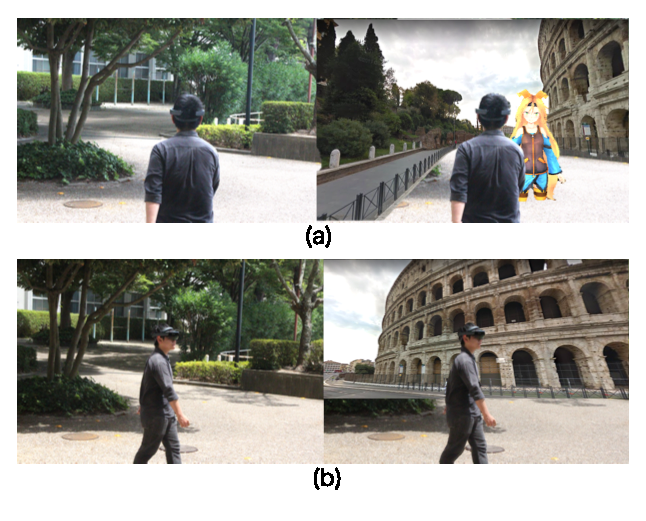
\includegraphics[width=11cm]{img/02_proposedmethod/user_dire.eps} 
\end{center}
\caption{(a)奥に向かい歩くと道が奥に続く.(b)歩く方向を変えると道が続く方向も変わる}
\label{figure:landscape_rotate}
\end{figure} 

%この時道路部分のみ現実の風景を表示することで,他の歩行者や乗用車などと衝突する危険を抑制する.
%重畳イメージを図\ref{figure:changescenery}に示す.
%図\ref{figure:changescenery}においてシステムを通してユーザがみている風景の道路部分は現実地風景の道路部分が表示されており,道路以外の部分は遠隔地の風景が表示されている.これによりユーザは現実の道路を視認しながら遠隔地の風景を楽しむことができる.
%本手法を実装するため遠隔地の風景を360度パノラマ画像として取得し,球体オブジェクトに貼り付けることでユーザの周囲の風景を変化させる.図\ref{figure:sphere}にローマのコロッセオの風景をパノラマ画像として取得し,球体オブジェクトを貼り付けた例を示す.














%従来睡眠を支援するアプリケーションは, 前述したとおり睡眠の質を向上させるものが多かった. 

%しかし, 2016年の研究で, 現代人の多くが自覚できない睡眠不足(潜在的睡眠不足)を抱えていることが明らかになった\cite{psd}.
%この原因として, 被験者の習慣的睡眠時間が必要睡眠量よりも平均1時間ほど短いことがあげられた.
%この問題の改善には, 睡眠の質のみならず量をも充足することが必要である.

%そこで我々は時計の時刻を操作し, ユーザが知覚する時刻を早めることで, 睡眠量を確保できるシステムを開発した.

%\subsection{IllusionClock}
%IllusionClock では, 表示デバイス及び管理アプリケーションの画面に表示する時刻(以下, 表示時刻)を, 実際の時刻よりも早めることにより, ユーザに表示時刻が正しいものだと錯覚させる.

%ここで, 現実ではユーザが理想とする就寝時刻である瞬間に, IllusionClock ではユーザの普段の就寝時刻を表示することで, 普段通りの生活を送ろうと考えたユーザの理想の就寝時刻と実際の就寝時刻とを近づけることが出来る.


%\subsection{生活リズム推定}
%IllusionClock ではユーザの普段の就寝時刻を推定し, 記録している.
%ユーザは加速度センサを搭載している AndroidWear を手首に装着する(図\ref{fig:wearable}). アプリケーションを起動し(図\ref{fig:system}), 普段通りの生活を送るだけで, 普段の就寝時刻が記録される.




%\subsection{時間変化設定}
%IllusionClockでは, 時刻変化の設定をユーザが Android アプリケーションを介して行う(図\ref{fig:setting}). ユーザが設定できる項目は理想就寝時刻, 普段の就寝時刻, 変化曲線である. 普段の就寝時刻に関しては生活リズムの推定結果を反映させることが可能である.

